\chapter{Alignment with tandem repeats}

Tandem repeat is a region in the genomic sequence that contain two or more
consecutive repetitions of the similar sequence.  Tandem repeats are important
for sequence alignment, since more than $2\%$ of the human genome is covered by
short tandem repeats, and they occurs in many genes and regulatory regions
\cite{Gemayel2010}. Additionally, recent short insertions in human genome are
mostly caused by tandem duplication \cite{Messer2007}.  Tandem repeats, like
other sequences, undergo evolution and therefore mutations, insertions, and
deletions occurs. Therefore individual copies of repeated sequence are not
exact.  Additionally, most of the tandem repeats evolved using tandem segmental
duplications, and therefore segments with tandem repeats contain variable
number of copies (not exact) of original segment. Aligning segments with tandem
repeats is hard, because it is not clear which copies of tandem repeat are
orthologous (created by speciation, not duplication within same genome).
Tandem repeat does not only affect quality of alignment within repetitive
segments, but error spread into adjacent columns of an alignment, as we show in
section \ref{}. \reformulate{Addtionally, comparative genomic methods are
sensitive to the quality of underlying alignment, and even ssmall inaccuracies
may lead to artifacts in the results of comparative methods.} \todo{Ujednot
oznacenie repeatov a poctu opakovani}

We introduce tractable model that explicitly accounts for tandem repeats. We
additionally use the maximum expected gain framework to explore several decoding
criteria for our model.

\todo{Co je to tandem duplication}

\todo{Priklad tandem repeatu a zleho zarovnania -- vyber nieco zo simulacie}

\section{Methods for aligning tandem repeats}

Alignment with tandem duplications were studied first by Benson
\cite{Benson1997}, who proposed extension of the Needleman-Wunsch
algorithm. In their scoring scheme, they scored duplications as an separate
event. Each duplication was penalized by duplication initiation cost,
duplication extension costs for each copy and Needleman-Wunsch like scoring
scheme to score original string with its repetitions. Time complexity of
resulting algorithm was $O(n^4)$ and Benson proposed heuristic algorithm to
compute alignment in reasonable time. \todo{Mozno to strosku rozsirit a dat
presnu formulaciu} Additional work was done by alternative incorporation of
tandem duplication (and other operations) into the scoring schemes
\cite{Sammeth2006, Berard2006, Freschi2012}, or using lossy compression scheme
that collapsed tandem repeats and aligning compressed sequences
\cite{Freschi2012}.

Traditional approach to deal with tandem repeats is to mask repeats in both
sequences and then aligned masked sequences by alignment algorithm of our
choice. Masking is replacing low complexity region (e.g. tandem repeats) either
with lower-case letters (soft-masking) or with N symbols (hard-masking, N
represents any base). Masking is done by method for finding tandem repeats,
such as \abbreviation{Tandem Repeat Finder}{TRF} \cite{Benson1999}, TANTAN
\cite{Frith2011}, mreps \cite{Kolpakov2003}, or ATRhunter \cite{Wexler2005}. 

Methods mentioned above were not probabilistic methods. The first probabilistic
method specifically targeting tandem repeats was introduced by Hickey and
Blanchette \cite{Hickey2011}. They developed context-sensitive model based on
pair Tree-Adjoining grammars, and taking into account that majority (roughly
$90\%$  \cite{Hickey2011}) are caused by tandem duplications.  Their model does
not explicitly model arbitrary number of copies of repetitive region, it
focused on short context sensitive indels caused by tandem duplications.  Time
complexity for their decoding algorithm was $O(n^2L^2)$, where $n$ is the
length of the sequences and $L$ is the maximal length of context sensitive
indels.

Another, not entirely probabilistic method was developed by Kováč {et. al
(2012)} \nocite{Kovac2012}. Aim of the method was to align repetitive motif
inside some protein families (for example zinc finger proteins), which are
similar to the tandem repeats. Their method focused on correctly aligning
individual occurrences of motifs. They combined profile HMM and pair HMM, and
developed new decoding algorithm similar to the Viterbi algorithm. Despite
usage of probabilistic models, their method was not probabilistic model. 

\todo{check ci to tak naozaj je}
\begin{reformulate*}
Hudek \cite{Hudek2010} developed algorithm that is mixture of the Viterbi and
posterior decoding. The algorithm was aimed to reduce the misalignments due to
short tandem repeats with the consensus length $1$, for example $u=AA$ in the
first sequence and $v=AAAAAAAAA$ in the second sequence. Algorithm developed by
Hudek was considering all possible alignments of $u$ and $v$ in the final
alignment. Algorithms goal was to segment alignment into blocks, such that each
block contain gaps in at most one sequence. The cost of the block was the sum of
the probabilities of all alignments of such block. The final alignments is
created from blocks by the Viterbi algorithm.
\end{reformulate*}

\section{Models and Methods Searching Tandem Repeats}

In this section we describe methods and models we used for improving
performance of our methods or as a parts of larger model for aligning sequences
with tandem repeats. 

\subsection{Tandem Repeat Finder}

Probably the most popular method for searching for tandem repeats is to use TRF
\cite{Benson1999}.  Tandem repeat finder find the position of tandem repeats,
consensus sequence (the pattern that is repeating), alignment of the consensus
sequence and the input sequence, and various other information about repeats.

Method consists from two components: detection and analysis. Detection
component tries to find a set of candidate tandem repeats by analyzing the
differences in the positions of matching $k$-tuples (subsequence of the input
sequence of length $k$). It uses several statistical criteria to detect repeats
and distinguish between tandem repeats and non-tandem repeats
\cite{Benson1999}.

Analysis component aligns candidate pattern using wraparound dynamic
programming \cite{Myers1989} with the surrounding sequence. If the alignment is
not successful (candidate pattern has to be aligned at least $2$ times to be
successful), candidate repeat is discarded. Otherwise, the consensus sequence
is computed from the alignment along with other statistics about tandem repeat.


Tandem repeats found by TRF can be redundant.  They can overlap, have slightly
different consensuses, the consensuses can be shifted cyclically, and can have
different lengths, as in following example:

\begin{verbatim}
Sequence  X:        CACCGCCACCACCGTAG
Consensus ACCACC:    ACCACCACCACC      2 repetitions
Consensus AAC:       ACCACCACCACC      4 repetitions
consensus CAC:      CACCACCACCACC      4.3 repetitions
\end{verbatim}

The sequence $X$ contain repetitive subsequence, and there are three possible
consensus sequences with different number of repetitions. Note that the
repetition of the consensus does not have to be full; as with the $CAC$
consensus where we have $4.3$ ($0.3$ stands for the last $C$ in the repetitive
sequence). This is important to know, because we will use the TRF to find
the set candidate repetitive regions of input sequences, not as the definitive
list of repetitive regions.

Note that the purpose of this example to illustrate redundancy of TRF output.
If we ran TRF on sequence $X$, the output would be only repeat with $CAC$ as an
consensus.

\subsection{Sunflower model}
\firstUseOf{Sunflower model} is HMM that models tandem repeats of one
previously specified consensus $C=c_1\dots c_k$. We developed it for our model
for aligning sequences with tandem repeats, but it can be also used as an
simple tool for searching tandem repeats (but it is highly likely that its
performance would be worse than TRF).

Sunflower is extension of profile HMM described in section \ref{HERD:METHODS}
in Figure \ref{FIGURE:PROFILEHMM} (page \pageref{FIGURE:PROFILEHMM}). Sunflower
models sequence of tandem repeats of single original consensus $C$. This model
assumes that repeats evolved independently from consensus $C$. One can think
about it as that at single point of time, sequence $C$ in genome was copied
several times, then resulting sequence undergo through simple evolution events:
substitution, deletions and insertions.

\begin{figure}
\begin{center}
\begin{subfigure}[b]{0.5\textwidth}
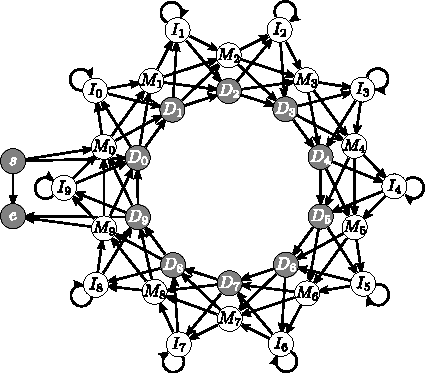
\includegraphics{../figures/SunflowerSilentCircle.pdf}
\caption{Cyclic profile model}\label{SUBFIGURE:SUNFLOWERSILENTCYCLE}
\end{subfigure}%
\begin{subfigure}[b]{0.5\textwidth}
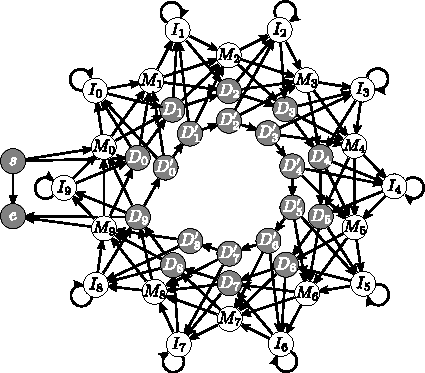
\includegraphics{../figures/Sunflower.pdf}
\caption{Sunflower model}\label{SUBFIGURE:SUNFLOWER}
\end{subfigure}
\end{center}
\caption[Example of the Sunflower model]{Example of the Sunflower model for
consensus of length $10$. White states emits one character and gray states are
silent states. States $s$ and $e$ are initial silent states. Sunflower model
has additional delete states $D'_0, \dots D'_8$ to remove silent cycle from the
model.}
\label{FIGURE:SUNFLOWERMODEL}
\end{figure}

To model this process, start with profile HMM for consensus $C$ and made it
cyclic: It contains states $M_0,\dots, M_{k-1}, I_{0}, \dots, I_{k-1}$ and
$D_{0}, \dots, D_{k-1}$. The transitions between the states are similar to
profile HMM:  $M_{i}\to M_{i\oplus 1}, M_i\to I_i, M_i\to D_{i\oplus 1}, I_i\to
I_i, I_i\to M_{i\oplus 1}, I_i\to D_{i\oplus 1}, D_{i}\to D_{i \oplus 1},
D_{i}\to M_{i\oplus 1}, D_{i}\to I_i$ for all $0\leq i < k$, where $\oplus$ is
$+$ modulo $k$. As in profile HMM, $D_i$ states are silent. Additionally we add
silent start state $s$ and silent end state $e$ with transitions $s\to M_0,
s\to D_0, D_{k-1}\to e, M_{k-1}\to e$ and transition $s\to e$ to model empty
tandem repeat.  Whole model topology is in Figure
\ref{SUBFIGURE:SUNFLOWERSILENTCYCLE}.

The problem with this model is that it contains cycle of silent states, which
causes problems with training and decoding algorithm, as was briefly mentioned
in section \ref{SECTION:SILENT}. We could remove these states, but we would
have to add additional $\theta(k^2)$ edges to by able to delete arbitrary (in
cyclic sense) parts of consensus cycle. Therefore we have decided to remove
transition between delete states $D_{k-1}$ and $D_0$. To compensate to the lost
possibility of deleting arbitrary part of tandem repeat, we add additional
chain of delete states $D'_0, \dots, D'_{k-2}$ that are accessible only from
state $D_{k-1}$ (by transition $D_{k-1}\to D'_0$ and their outgoing
transitions are similar to delete state transitions: $D'_{i}\to M_{i+1},
D'_{i}\to I_i$ for $0\leq i\leq k-2$ and $D'_{i} \to D'_{i+1}$ for $0\leq i <
k-2$. Full model is in Figure \ref{SUBFIGURE:SUNFLOWER}. We call this model the
\firstUseOf{Sunflower} model.

\todo{Premenuj end state na final state, vsade!} This model has $4k+1$ states
out of which $2k+1$ are silent, and $12k+1$ transitions. Since alphabet size is
$4$, there are $14k+2$ parameters to train for a consensus $C$ (including
emissions of insert and match states). Models with large number of parameters
are hard to train, so we reduce the number of parameters. We bind similar
transitions so that they have the same probability.  We ended with parameters
$p_{ab}$ where $a,b\in \{m, i, d, \cdot\}$. $m$ stands for any match state, $i$
stands for any insert state, $d$ states for any delete state (from both
chains), and $\cdot$ is either start or end state. Therefore probability of
transition from match state to delete state is $p_{md}$ and probability of
transition from insert state to final state is $p_{i\cdot}$.  Probabilities
were set in a way, that $\sum_{b\in\{m,i,d\}p_{ab}}=1$ for all possible $a$.
Therefore, transitions from $M_{k-1}, D_{k-1}$ and $D'_{k-1}$ does not sum to
$1$, because they are either missing one transition of having one additional
transition. Therefore for those states the probability of transitions were
multiplied by constant so that they form probability distribution.
\todo{Skontroluj ci tu nie su nejake vynimky}

Emission parameters were reduced in following way: all insert states shared
same emission distribution. For emission distribution of match state $M_i$ we
assumed that base from consensus $c_i$ evolved over evolutionary time $t$
according to Jukes-Cantor model. This model is theoretical model of evolution
that assumes constant rate of evolution. Under this model base $B_1$ evolved
over time $t$ to different base $B_2$  with probability $1/4(1-\exp(-4t/3))$.
The probability that $B_1$ after time $t$ will be again $B_1$ is
$1/4(1+3\exp(-4t/3))$ \cite{Durbin1998}. Time $t$ was same for all match
states. Therefore emissions of all states has only $4$ parameters ($1$ for
match states and $3$ for insert states).

\begin{note}
In Jukes-Cantor model, the parameter $t$ is not time as measured by
seconds/years. It is a branch length in evolutionary tree and it is
multiplication of substitution rate and time. We used this small inaccuracy to
simplify explanation.  More details can be found in \cite{Durbin1998}.

\end{note}

Sunflower model models only tandem repeat and it is not directly usable for
finding tandem repeats. To do so, we have to alter this model. Let $S_C$ be the
Sunflower for consensus sequence $C$. Then we create model consisting of state
$B$, that model non-repetitive part of the sequence with model $S_C$ with an
transition $B\to s$ with probability $p_r$ which is the probability of repeat
starting at particular position in the sequence and with transition $e\to B$
with probability $1$. There is also transition $B\to B$ with probability
$1-p_r$. Afterwards, we can use the Viterbi algorithm with this model to find
all of the occurrences of tandem repeat with consensus $C$. However, with this
model we can search only for specific repeats. This model will be used as an
submodel for aligning sequence with tandem repeats in section
\ref{SECTION:REPMODELS}.


\subsection{TANTAN}

\firstUseOf{TANTAN} is high-order HMM aimed for finding tandem repeat developed
by Frith \cite{Frith2011}. Unlike Sunflower model, TANTAN models tandem repeats
with arbitrary consensus. Its only restriction is the maximal length of the
repeated motif $k$. TANTAN is aimed at finding tandem repeats. Here we describe
only the core of the model; the part that models tandem repeats. The core of
the model can be transformed to the model usable for search by same method as
we described for Sunflower model.

\begin{figure}
\begin{center}
\begin{subfigure}{0.19\textwidth}
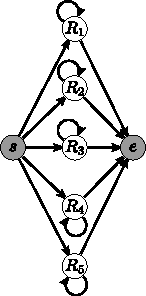
\includegraphics{../figures/tantan_simple.pdf}
\caption{Simple model}\label{FIGURE:TANTAN:SIMPLE}
\end{subfigure}%
\begin{subfigure}{0.3\textwidth}
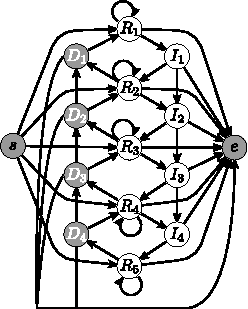
\includegraphics{../figures/tantan_indel.pdf}
\caption{With indels}\label{FIGURE:TANTAN:INDEL}
\end{subfigure}%
\begin{subfigure}{0.35\textwidth}
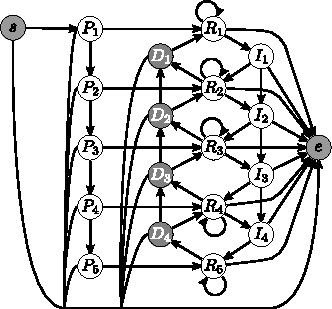
\includegraphics{../figures/tantan_init.pdf}
\caption{With first repetition}\label{FIGURE:TANTAN:INIT}
\end{subfigure}%
\end{center}
\caption{Three variants of the core of the TANTAN model. Gray states are
silent. The first one is simplified model, only with repeat states. The second
one is one used by Frith \cite{Frith2011} allowing insertions and deletions.
Last one is our extension with additional state $P_1, \dots P_5$ that models
first occurrence of repetitive sequence.}\label{FIGURE:TANTAN}

\end{figure}

Main idea is to use state of order $l$ to model repeats with consensus length
$l$. If we have high-order state of order $l$ and want to generate $i$-th
symbol of sequence $X$, standard high order state of order $l$ depends on
subsequence $X[i-l:l]$. TANTAN's states of order $l$ depends only on symbol
$X[i-l]$. Model consists from $k$ high-order states $R_l$, $1\leq l\leq k$
called repeat states, where state $R_l$ is of order $l$. Emission of state
$R_l$ is set in such way, that state emits same symbol as $X[i-l]$ with high
probability. By adding transition $R_l\to R_l$ we obtain HMM modeling tandem
repeats without indels with consensus length $l$. By connecting states
$R_1,\dots, R_k$ to single start and end state as show in figure
\ref{FIGURE:TANTAN:SIMPLE} we obtain HMM that models repeats with consensus
lengths $1$ through $k$.

This model however does not allow insertions and deletions from the model. This
can be done similarly to the profile HMMs by adding insert states $I_1,\dots,
I_{k-1}$ and silent delete states $D_1, \dots, D_{k-1}$ connected as in the
Figure \ref{FIGURE:TANTAN:INDEL}. There are however slight differences with the
profile HMM.  In profile HMM, delete states were used to skip at least one
match state, while in TANTAN delete state is used move to state with lower
order. Additionally, insert states moves in opposite direction, using insert
state causes increase of the order of the repeat state. It is also possible to
move from insert state $I_{j}$ to insert state $I_{j+1}$ which is not possible 
in the profile HMM.

One disadvantage of this model is that it does not model the first occurrence
of the consensus sequence, since repeat states model only the repetitions of
the sequence. This was problem when we wanted to incorporate TANTAN into our
model. Therefore we added additional chain of prefix states $P_1,\dots, P_k$
modeling first repetition. Transitions are now only to end state (modeling
empty sequence) and state $P_1$. State $P_l$ has transitions to the end state,
repeat state $R_l$ and the state $P_{l_1}$ (if such state exists).

%Emisie a sme hotovy
We set emission distribution of the insert and prefix states to the background
probability: the distribution of the bases in DNA. Emission state of the state
$R_l$ was derived using Jukes-Cantor model with parameter $t$. \todo{spresni}

\section{Models for Aligning with Tandem Repeats}\label{SECTION:REPMODELS}
\todo{Mozno chceme aj niekde popisat ake mame ciele}
In this section we describe models that we have used in our methods. We
describe it in an dual way. As an generalized PHMM and later we extend it into
equivalent PHMM (emissions length are at most $1$ in all sequences).
Equivalency is in the way, that distribution of generated alignments and
annotations are same.

Generalized model is obtained by taking simple three state HMM model from
section \ref{} and adding single generalized pair state $R$, called
\firstUseOf{repeat state}, that in single step generates whole tandem repeats
in both sequences. Since $R$ state can in theory generate arbitrary long
sequences, while decoding using this model, $R$ state does not produce
alignment of bases of tandem repeats. Its aim is to filter tandem repeats out
of alignment so that they do not cause biases in the alignments formed by other
states (match and indel states). To realign those parts later in
post-processing step. The overall topology of GPHMM is illustrated in figure
\ref{FIGURE:REPEAT_GENERAL}.

To made this model flexible, emission distribution of $R$ is defined by
additional PHMM. Since repetitive sequences in tandem repeat are very similar
to each other, we did not try to model the evolution of repetitive part of the
sequence. We assumed that repeats generated by one emissions of $R$ originates
from single consensus sequence and were developed independently. Model was
constructed from sunflower models. Let $C$ be the set of all consensuses that
we want to model. For each consensus $c\in C$ we created sunflowers $S_c^X$ and
$S_c^Y$.  $S_c^X$ is pairwise sunflower model with consensus $c$ that generates
symbols in sequence $X$ and nothing in second sequence. $S_c^Y$ is analogous.
We connect $S_c^Y$ after $S_c^X$ and thus getting model $H_c$ that generates
repeats in both sequences. We connected models $H_c$ for $c\in C$ in parallel
by single start and single end state as in figure \ref{FIGURE:REPEAT_GENERAL}.
The probability from start state to model $H_c$ was determined from posterior
distribution of consensuses $\prob{c}$. Note that the size of this model is
determined mostly by the size of set of all consensuses and therefore this
model can be very large, even infinite if we consider all possible sequences as
an possible consensus for an repeat. To keep the model size small we used
program TRF to compute a set of candidate consensuses $C$ and use it for
construction of model.  We call this generalized model \abbreviation{sunflower
field}{SFF}.

\begin{figure}
\begin{center}
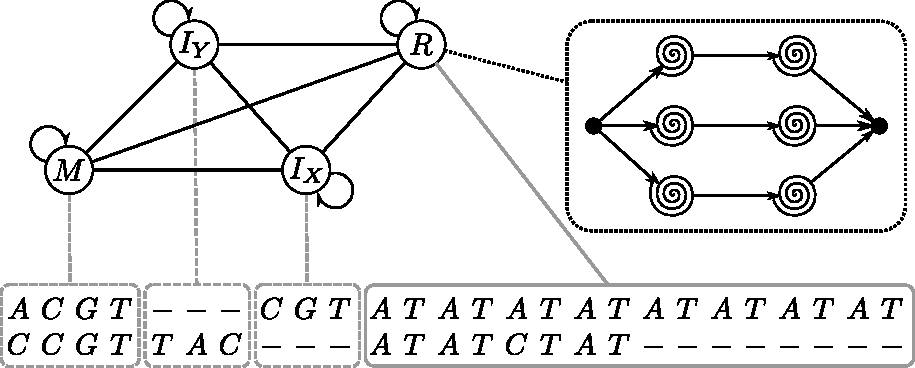
\includegraphics[width=14cm]{../figures/PairRepeatHMMGeneral.pdf}
\end{center}
\caption[General topology of Repeat PHMM]{ 
Topology of Repeat PHMM. We extend 3-state PHMM with one generalized states
$R$, that in one emission generates tandem repeats in both sequences. The
emission distribution of $R$ state is defined by another PHMM. Gray lines
represents emissions: dashed lines corresponds to multiple emissions from same
states, while full line represents one emission. Dotted black line represents
connection to submodel that is used for generating tandem repeats.

Black states in submodel on the right are silent start and end states. Spirals
represents submodels generating tandem repeat in one sequence. They are in
pairs of two identical models, one for generating tandem repeat in one
sequence, other for generating tandem repeat in other sequence. There are
multiple pairs of submodels, each for modeling different consensus.

 }\label{FIGURE:REPEAT_GENERAL} 
\end{figure}

We also experimented with using TANTAN-like model in construction of PHMM
defining emissions distribution of state $R$. Since TANTAN model does not model
the first repetition, we have added chain of states $I_1, \dots, I_n$ to model
first repetition.  Similarly as with sunflowers, we created two copies of
TANTAN, each generating repeats in only one sequence and connect them together
exactly as we would connect sunflowers. Since TANTAN model does not rely on
consensus, it is not necessary to create more copies of TANTAN HMM and it's
general topology looks like SFF's with only one consensus. Since TANTAN is high
order HMM, resulting model is high order and generalized pair HMM. We refer to
this model as \abbreviation{TANTAN PHMM}{TTP}. Advantage of this model over SFF
is in it's size, since TTP will have in practice less states than SFF. However
in TTP, does not satisfy assumption that repeats origins from single consensus,
since each repetitive element is created from previous occurrence and repeats
in sequences $X$ and $Y$ are independent of each other. \todo{obrazok?}

While having SFF or TTP defined as an $4$ state hight order GPHMM might be
convenient for some decoding methods, in general using generalized models
increase time complexity of decoding algorithms quadratically. Therefore we
also worked with their expanded versions: we removed state $R$ and replace it
with model generating repeats (referred as a submodel). All transitions
entering originally into $R$ were directed to start state of submodel and all
outgoing transitions from $R$ now start in end state of submodel. Distributions
of alignments generated by this PHMM has clearly not changed. Additionally, if
in original GPHMM we used identity function as an labeling function
$\lambda_{ID}$ and in expanded model we label states from submodel by label
$R$, resulting in labeling function $\lambda_R$, distribution on annotations
on alignments has also not changed. \todo{toto znie ako od hotentota}

For consensuses in SFF model, we use $310,091$ motifs found by TRF program run
on the human chromozome 15 and its orthologous sequences in the dog genome. The
probability of choosing particular consensus was the observed frequency of the
consensus in the TRF output. In practice, we limit the Sunflower submodels only
to those which was found by TRF in the input sequence.  Additionally, the input
sequence contain motif that is not in predefined set, we add it to the model
with the probability of the least occurring motif in the model (this is necessary
if we run our model on sequences that are not sampled from the model).

We set parameters of the Sunflower submodel manually: the insert and delete
rates were set to $0.005$, the match states allows mutations from consensus
according to the JC model with parameters $t=0.05$.
\todo{Ako je definovana pravdepodobnost emisie?}
Parameters of the TANTAN submodels were estimated by the Baum-Welch algorithm
\cite{Durbin1998} on 500 repeats sampled from SFF.

The size of the TTP model depends on the length of the longest possible
consensus TODO, while the size of the SFF model depends of the total lenght of
all consensuses used. Therefore SFF can be exponentially larger than TTP model.
On the other hand, SFF model models assumes that consensuses were developed
independently, while the TTP model assumes that repetition evolves from the
previous occurrence of the repetition.

While decoding methods are Tandem repeats at orthologous positions in two
species may share common ancestor and therefore share part of their evolutionary
history. However, it is possible that they were consequently modified by
additional evolution events after speciation (including more tandem
duplications). In our model we ignore such complex evolution of repeats, because
modeling it would lead to very complex model and increase the difficulty in
decoding and training. Kováč {\it et. al} developed method added limited
dependence by adding repeat submodels emitting copies in the two sequences at
same time \cite{Kovac2012}.


\section{Decoding methods}

In this part we describe several optimization criteria we have used. We used
following optimization criteria: the Viterbi algorithm (VA), the
posterior decoding (PD), the marginalized posterior decoding (MPD), block
Viterbi algorithm (BVA) and block posterior decoding (BPD). The first three
methods we used with expanded models, the latter two methods we used with
generalized version of the model. We have already described first three
algorithm in section \ref{}. Here we introduce the highest expected gain
framework for pair HMM and formulate used algorithms using gain
functions.\todo{Mohol by si zacat pouzivat tieto skratky}

To be able to use highest expected framework, we will represent alignment using
\todo{uprav indexy}
indices to sequences. We will also include the state that generated that
symbols (or it's annotation). In case of generalized models (can generate more
than one columns), only the first column will contain state, other columns will
contain symbol $\varnothing$. We will call this structure annotated alignment.
Formally, annotated alignment of length $t$ will of sequences $X=x_0x_1\dots
x_{n-1}$ and $Y=y_0y_2\dots y_{m-1}$ will be represented as sequence of tuples
$(u_0, a_0, b_0), \dots, (u_{t-1}, a_{t-1}, b_{t-1})$ where $a_i\in \{0, \dots,
{n-1}\}\cup\{-_0, \dots, -_n\}$ and $b_i \in \{0, \dots, m-1\}\cup\{-_0,
\dots, -_m\}$, and $u_i$ is either annotation symbol or symbol $\varnothing$.
Number $i$ represents $i$-th symbol in respective input sequence and $-_i$
represents gap in the sequence before position $i$ (if $i$ is the length of the
sequence, it represents the gap at the end of the sequence). For example $(47,
-_{42})$ means that $x_{47}$ is aligned to gap that is between $y_{41}$ and
$y_{42}$.  Naturally, indices in $a_i$ and $b_i$ have to be non-decreasing,
each non-dashed symbol can be in the alignment only once.  Naturally, $a_0$ has
to be $0$ or $-_{-1}$, $a_t$ is $n$ or $-_m$. The constrains for $b$ are
analogous. Additionally, $u_0\not=\varnothing$ and if some $u_i$ is equal to
$\varnothing$ then such column was emitted by same emission as previous column.
If we use non-generalized model, the annotated alignment will not contain
symbol $\varnothing$. The reason for using annotation symbol is that we will
need to be able to distinguish between different generalized emissions. We can
define probability of annotated alignment $\Lambda$ as the sum of of the
probabilities of the state paths that generate such alignment and it's
annotation is equal to annotation from $\Lambda$. We denote this probability as
$\prob{\Lambda\mid X, Y}$. We will refer to triple $(u_i, a_i, v_i)$ as an
\firstUseOf{annotated alignment column}.

We will be interested in \firstUseOf{repeat annotation}, where annotation
function $\lambda_R(u)$ is $R$ if state is $R$ state (or was created from $R$
state in the expanded version of the model) and $u$ otherwise (for match,
insert and delete state). Repeat annotation $\lambda_R$ is equivalent to
identity function for 3-state HMM that does not explicitly model repeats.
The probability of a state path and annotation is defined exactly as for HMM
that generates only one sequence.

Similarly as with regular HMMs, we can define gain functions for annotation
$G(\Lambda, \Lambda')$ that corresponds to ``similarity'' of two annotated
alignments.  Since PHMM define probability distribution $\Lambda_T$ of the
correct annotated alignments, we can define the expected gain of annotated
alignment given sequence $X$ and $Y$ and gain function $G$:
\todo{uprav oznacenia tak, aby boli konzistentne s obycajnymi HMM}
\begin{equation}
E_{A_T}\left[G(\Lambda, \Lambda_T)\mid X, Y\right] = 
\sum_{\Lambda_T}G(\Lambda, \Lambda_T)\prob{\Lambda_T\mid X, Y}
\end{equation}

Since we do not know the correct annotated alignment, we search for the
annotated alignment $\Lambda^*$ with the highest expected gain:

\begin{equation}
\Lambda^* = \arg\max_AE_{A_T}\left[G(\Lambda, \Lambda_T)\mid X, Y\right]
\end{equation}

Now we express optimization criteria of decoding methods we use within this
framework. 

\paragraph{The Viterbi decoding and block Viterbi decoding} Gain $G_V(\Lambda,
\Lambda_T)$ function for the Viterbi algorithms assigns $+1$ if the predicted
annotated alignment $\Lambda$ is identical to true annotated alignment
$\Lambda_T$. Optimization algorithm for non-generalized model was described in
the section \ref{}.  The time complexity run in time $O(nmE)$ where $E$ is the
number of non-zero transitions in the model.  We will discuss the time
complexity for the block Viterbi decoding in the end of this section.

We will make distinction between the Viterbi decoding and block Viterbi
decoding when using SFF or TTP models. Using the Viterbi algorithm on the
expanded model will be referred to as the Viterbi decoding. Using the Viterbi
algorithm on the generalized version of the model will be referred as the block
Viterbi decoding. The difference between these two versions is that in the
Viterbi decoding, we account only one state path through the repeat submodel.
The block Viterbi decoding however sum all possible paths through the repeat
submodel and therefore abstract from exact realization of the alignment of
repetitive sequences.

\paragraph{Posterior decoding}
In the Viterbi algorithm, the non-zero gain is awarded only if an annotated
alignment is entirely correct. Gain function $G_P$ of posterior decoding (which
was defined in section \ref{})is more gradual. It assigns $+1$ for every
correctly predicted annotated alignment column. Annotated alignment column
$(u_i, a_i, b_i)$ is correctly predicted if there is alignment column $(v, a_i,
b_i)$ for arbitrary $v$ in the true annotated alignment (posterior decoding
ignored labels). 

We will consider stricter version of the posterior decoding by adding
additional condition: the corresponding annotated alignment column in the
correct annotated alignment has to have same annotation; $\Lambda_i$ has to be
equal to $\Lambda_{Tj}$. This stricter condition is aimed for the expanded
versions of SFF and TTP, since otherwise it would treat repeats as gaps despite
having orthologs in the other sequence (our models treat such repeats
independently and models them formally as gaps).  For the 3-state HMM, this
stricter condition does not have effect. Note that we use this decoding only
with expanded versions of SFF and TPP or with 3-state model.  The running time
of the posterior decoding is again $O(nmE)$.

\paragraph{Marginalized posterior decoding}

Marginalized posterior decoding (gain function $G_M$) is similar to the
posterior decoding. The only difference is that we treat all gaps to be
identical despite their position in the sequence. Therefore we treat column
$(u, i, -_j)$ to be same as $(u, i, -_k)$ (gaps in other sequence are treated
symmetrically). The optimization of this gain function is almost identical to
optimization of $G_P$. Only difference is that after computation of the
posterior probabilities, we replace probability $(u, i, -_j)$ with the sum of
$(u, i, -_l)$ of all $l$. The algorithms has also time complexity $O(nmE)$.  As
with posterior decoding, this decoding method is not used on the generalized
models.

\paragraph{Block posterior decoding}
\todo{numvber of emitted symbols -> number of emitted non-gap symbols}
Block posterior decoding is version of the posterior decoding for generalized
models. In block posterior decoding we score emissions instead of independent
columns. In particular, for SFF and TTP models columns from states $M$, $I_X$
and $I_Y$ are scored exactly as in the posterior decoding, since those state
emits only one column. Column $(u_i, a_i, b_i)$ gets $+1$ if in the true
alignment exists exactly same column and $u_i\in\{M, I_X, I_Y\}$. Emission from
state $R$ in form of $\Lambda_E=(u_i, a_i, b_i)(\varnothing, a_{i+1},
b_{i+1})\dots (\varnothing, a_{j}, b_{j})$ where $(j+1)$-th column does not
contain $\varnothing$ get score $+l$ where $l$ is the number of emitted
characters in the emission $\Lambda_E$ is in the correct annotation is emission
of state $u_i$ that emit exactly same set of position symbols.  The reason for
using $+l$ instead of $+1$ is that it would be better not to use $R$ state,
because its long emission get score $+1$ while same region would get higher
score when columns would be scored independently. Instead of $l$, the number of
emitted bases, we could use the number of emitted columns. However we would
then discriminate the submodels that would tried to align repeats (although we
did not used such model). Example of this gain function in in the Figure
\ref{FIGURE:BLOCK_POSTERIOR}.

\begin{figure}
\begin{center}
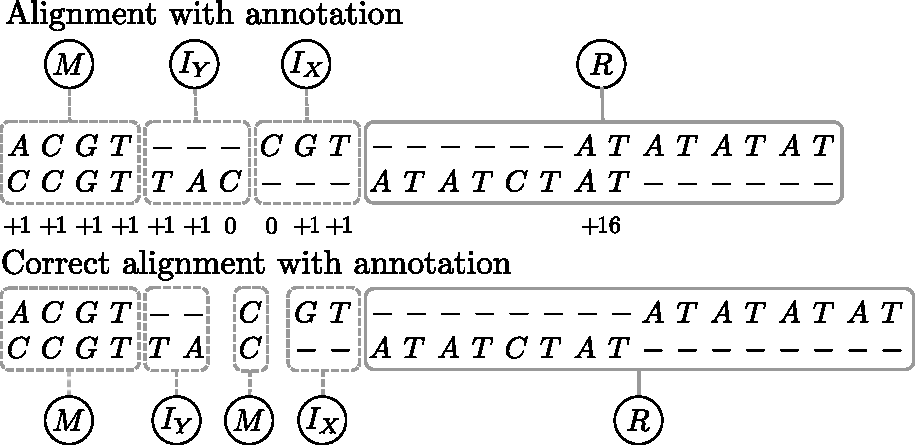
\includegraphics[width=14cm]{../figures/BlockPosterior.pdf}
\end{center}
\caption[General topology of Repeat PHMM]{ 
Explanation of block decoding gain function. Gray solid lines represents single
emissions, dashed lines represents multiple emissions (each alignment column is
one emission). Emission from repeat state have gain $+16$ because it emits same
set of $16$ bases from correct positions as does repeat state in the correct
alignment. Other alignment columns get $+1$ only if there is same alignment column
in the correct alignment that was generated by same state.

}\label{FIGURE:BLOCK_POSTERIOR} 
\end{figure}

To optimize this gain functions, we have to compute posterior probabilities for
all emissions. In generalized PHMM, emission is given two intervals; one in the
sequence $X$ and one in the sequence $Y$. The number of possible emissions is
$O(n^2m^2)$. The expected gain of the emission is the posterior probability
multiplied by the number of emitted symbols. After computing expected gains of
individual blocks we can compute the highest scoring annotated alignment in
$O(n^2m^2)$ time.

Let $E$ be the number of transitions in the repeat submodel. The naive
computation of the expected gain for the pair of intervals of length $n'$ and
$m'$ can be computed $O(n'm'E)$ by forward algorithm for generalized pair HMM,
which would lead to $O(n^3m^3E)$ algorithm for computing posterior
probabilities by forward-backward algorithm. By using proper preprocessing that
can be done in $O((n^2+m^2)E)$ time, we can lower the time complexity of
computing expected gain for an pairs of interval to $O(k)$ where $k$ is the
number of sunflower submodels (in case of TTP, $k=1$).

Let consider the repeat submodel $R$ with $k$ sunflower pairs $S^X_1, S^Y_1,
\dots, S^X_k, S^Y_k$. Let $p_i$ be the probability of entering sunflower
$S^X_i$.  The probability of transition from $S^X_i$ to $S^Y_i$ is $1$. We can
write the probability of generating sequences $X'$ and $Y'$ by submodel $R$ as
\begin{equation}
\prob{X', Y'\mid R} = \sum_{i=1}^k p_i\prob{X'\mid S^X_i}\prob{Y'\mid S^Y_i}
\end{equation}
By pre-computing all of the term $\prob{X'\mid S^X_i}$ and $\prob{Y'\mid
S^Y_i}$, we can compute the posterior probability of the emission in $O(k)$
time. Naive computation of all $\prob{X'\mid S^X_i}$ would take $O(n^3E)$ time,
but this can be further improved. When computing $\prob{X'\mid S^X_i}$ using
the forward algorithm, we can use the values from the forward table to compute
the probability of emitting any prefix of $X'$ by looking at the value in the
final state in the corresponding column of the forward table (In case of the
model without final state, we sum the probabilities in the corresponding
column). Using this, we need to run forward algorithm only for sequences
$X[i:]$ for all $0\leq i< n$. The optimization for the other sequence is
analogous. By using these techniques we can pre-compute the emission terms in
$O((n^2+m^2)E)$ time. Therefore the overall time complexity of the Block
posterior decoding is $O(kn^2m^2 + (n^2+m^2)E)$. By same techniques we
can optimize the block Viterbi decoding with same time complexity.

\section{Optimizations}

In this section we summarize additional techniques we have used to decrease
running time of decoding algorithms. The fastest decoding algorithms described
above run in $O(nmE)$ time, which is still prohibitive for longer sequences.
Additionally, block-based methods are even slower, so we need to use techniques
to speed them up. We used following optimizations:
\begin{itemize}[itemsep=-1mm]
\item We implemented standard technique of banding. We restrict the alignment
to window around guide alignment, that can be obtained by faster but less
precise alignment algorithms. We used Muscle\cite{Edgar2004} with default
parameters to compute guide alignment. The final alignment methods were
restricted to be within 30 bases from the guide alignment. This technique
reduce the $O(nm)$ term from the time complexity to $O((n+m)d)$ where $d$ is
the distance from the guided alignment.

\item The size of the SFF model is enormous. It is not practical to use model
with $310,091$ sunflower pairs. Therefore we used TRF program \cite{Benson1999}
to find consensus motifs in the input alignment and used only those to build
SFF model. Note that the transition probabilities to sunflower pairs were kept
same as in the original model. In case that TRF did find consensus that was not
in the original set of consensuses, we assign it the probability of the least
occurring consensus from the original set. This technique was not applicable to
TTP model.

\item To further reduce running time of the block Viterbi decoding and block
posterior decoding, we restrict the intervals where the generalized state could
emit sequences. We used repeat finders to get the list of possible intervals of tandem repeats in both sequences. Then we have
\todo{Tu som TERAZ!}

When using generalized models, time complexity of the decoding methods is
very large.  Therefore to compensate for this drawback, we used TRF program to
get list of candidate intervals where tandem repeats could occur. We use this
intervals to restrict parts of the sequence where the repeat state $R$ could be
used. Since TRF tool is not perfect in finding tandem repeats, ...

\end{itemize}

\section{Experiments}
\begin{reformulate*}
Ako sa generovali data, ako sa trenovali modely, ake miery sledujeme.  Bolo by
zaujimave sa pozriet ako porovname s hladanim tandemovych repeatov ak pouzijeme
TRF, alebo sunflower.

\end{reformulate*}


This section summarizes the details of this experiment and measures we were
using for evaluation. We evaluate our model using simulation experiments.  We
estimate parameters of the model using human-dog alignment (we annotated
alignment columns using TRF). Parameter for 3-state model and 3-state submodel
and transitions to the repeat state were therefore fully supervised.
We set the parameters of the Sunflower submodel to TODO

We sampled 200 test alignments each of length at least 200 bases \todo{check}
from the SFF submodel with the condition, that the number of repetitions in the
tandem repeat has to be at least three in at least one of the sequences. Reason
for this condition is that we want to prevent fake tandem repeats ( sequences
that are from the tandem repeat submodel, but are not in tandem repeats since
they are only repeats) which would not be detected by TRF.

We used same model for evaluation of parameters. To evaluate the robustness of
our model, we assess the effects of misspecification of parameters by
estimating model parameters from human-chicken alignment and perturbing model
parameters (details are in next section). Mreps was trained of the 200 separate
alignments sampled from the model. 

\paragraph{Measures:} The first measure we use was the error rate on the
alignments: number of incorrectly predicted columns of an alignment. Other
measures we investigate were measuring precision of repeat annotation.
Therefore we were measuring the specificity and sensitivity of repeat labeling
of columns and specificity and sensitivity of identifying the correct repeat
blocks; repeat block is maximal consecutive sequence of columns that are
annotated as repeat. Block must have been identical to be counted as an
correctly predicted.

Another measure we were using is the relation of the error rate and the
distance from the nearest repeat. Alignment column was considered as repeat if
in the correct alignment at least one base of the column was annotated as an
repeat. The distance is measured by the number of columns. This measure is more
important, because it illustrate the effect of SFF-like model. In the parts
that are distant from repeats, we do not expect improvement in the error rate
over the 3-state model, but we expect to improve alignments around tandem
repeats. 

\section{Results of simulation experiments}

\begin{reformulate*}
In this section we discuss the results of the simulation experiment. The tables
\ref{TABLE:SFFMAIN}, \ref{TABLE:SFFMAINORIGINAL},
\ref{TABLE:SFFOTHER},\ref{TABLE:SFFMARGINALIZED}, \ref{TABLE:SFF3STATEMASK},
and Figure \ref{FIGURE:SFF_GRAPHS}. 

We used 3-state model with Viterbi algorithm as the baseline method.

Nechcem este skusit spravit block marginalized posterior?
\end{reformulate*}



Using SFF model leads to decrease of the alignment error by $15-30\%$ as
opposed to baseline method as can be seen in table \ref{TABLE:SFFMAIN}. The
$15\%$ decrease was obtained just by replacing 3-state model with Sunflower
Field model, other improvements were made through using different decoding
algorithms; leading with the marginalized posterior decoding. The Viterbi based
methods had higher error rate than posterior based methods and the
block-versions decreased error rate only slightly. Surprisingly, block based
methods had poorest performance in the block sensitivity and specificity and
repeat sensitivity, because these measures are closer to what those methods
optimize. Reason for this is perhaps due to \reformulate{intervals obtained
from TRF}. This can be backed up by table \ref{TABLE:SFFMAINORIGINAL}, where
all of the algorithms used correct intervals and consensuses. As we see, in
these metrics the use of the correct intervals improved performance.

Similar behaviour was obtained for TTP model; using the original intervals, TTP
model has only slightly worse error rate than SFF, which is expectable, since
the data were generated from the SFF model. However, using TRF for intervals,
TTP has significantly higher error rate, which means that TANTAN is even more
sensitive to the intervals that are used. 

Table \ref{TABLE:SFFOTHER} contain other algorithms for sequence alignment. Namely, 
there is mreps tool\cite{}, which has even  TODO

It could be argued, that using same model for training and testing is not
\reformulate{good}. We have therefore make changes to model to demonstrate
robustness of our method. SFF model have two principal types of parameters;
parameters of the 3-state HMM and parameters of the Sunflower model. We
investigate the effect of \reformulate{misspecification} for both types
independently. For parameters of 3-state model, we have estimate parameters
from human-chicken alignments instead of human-dog alignment. For the second
type, we have perturbed the parameters of Sunflower model randomly by at most
$0.05$. On these models we run marginalized posterior decoding. The results are
in the table \ref{TABLE:SFFMARGINALIZED}.

Last we were investigating using different repeat finding
algorithm for masking methods. We used for masking correct intervals, Sunflower
model (modified for finding tandem repeats as described in section \ref{}),
TRF, and TRF with non-overlapping repeats (we select maximal scoring
non-overlapping set of tandem repeats out of TRF output). We used soft-masking;
we replaced masked bases with N symbol, that represents unknown base. For
decoding we used both the Viterbi and the posterior decoding. Results are in
table \ref{TABLE:SFF3STATEMASK}. Apart from  using correct intervals, the best
performing masking was used with non-overlapping repeats from TRF.

Additional metric we were investigating was the relation between error rate and
the distance from the nearest repeat. Figure \ref{FIGURE:SFF_GRAPHS} contains
graphs for this metric for various combination of parameters. In general, all
algorithms has highest error rate near borders of the repeat, with the error
rate lowering with the distance from the repeat. Most methods reach the
baseline error rate within distance $10$ bases of the repeat border.

Since we run many combinations of the model and algorithm, we can observe their
effect on error rate near repeat borders. Figures \ref{FIGURE:SFFOVER} and
\ref{FIGURE:SFFOTHER} suggests that decoding can improve error rate near
repeats, but most of the drop in the error rate was caused by using SFF model.
As with previous metrics, TANTAN with correct intervals performs similarly to
SFF model, however, its error rate near repeat raises significantly where
intervals were obtained from TRF (see Figure \ref{FIGURE:SFFTANTAN}). Using
incorrect model did not have large effect also on this metric as we can see in
the Figure \ref{FIGURE:SFFWEIRD}. Figure \ref{FIGURE:SFFBLOCKS} shows that when
comparing block method, using block Viterbi double the error rate near repeat.


\begin{reformulate*}
Tabulky, grafy, ... -- presnejsie tabulka, graf
\end{reformulate*}
\def\M{$^\circ$} % mark by a star
\def\MM{$^{\circ\circ\circ}$} % mark by two stars
\def\D{$^{\circ\circ}$} % mark by dagger
\def\DD{$^{\dagger}$} % mark by dagger
\def\R{$^{\yen}$}
\def\RR{$^{\yen\yen}$}
\def\CC#1{\multicolumn{1}{c}{#1}} % center column
\def\S{$^{\star}$}
Additionally to the variants of the method above, there are additional variants
of the model and algorithms, here is the set of marks that will be used to
distinguish between them.

\begin{itemize}[itemsep=-1mm]

\item[\M] method uses the real consensus motifs. 

\item[\D] method uses intervals from the real repeat blocks.

\item[\MM] method uses the real consensus motifs and intervals from the real
repeat blocks.

\item[\R] Parameters for the three-state submodel were estimated from
human-chicken alignment. 

\item[\RR] Parameters for SFF submodel were perturbed randomly.

\item[\DD] Columns with at least one masked character are considered as
repeats.

\item[\S] Non-overlapping set of repeats from TRF output with maximal total
score is used.

\end{itemize}

\begin{table*}
\begin{center}
\begin{tabular}{lr@{\quad}rr@{\quad}rr}
\hline
          & \CC{Alignment} & \multicolumn{2}{c}{Repeat} & 
\multicolumn{2}{c}{Block}\\
Algorithm & \CC{error} & \CC{sn.} & \CC{sp.} & \CC{sn.} & \CC{sp.} \\
\hline
\hline
%\hline
3-state Viterbi (baseline)    & 4.78\% \\
\hline
SFF marginalized    & {\bf 3.37\%} & {\bf 95.97\%} & 97.78\% & {\bf 43.07\%} & 44.87\%\\
SFF posterior       & 3.53\% & 95.86\% & 97.87\% & 42.70\% & 47.37\%\\
SFF block           & 3.51\% & 93.09\% & {\bf 98.07}\% & 36.50\% & 41.67\%\\
SFF block Viterbi   & 3.91\% & 93.26\% & 97.96\% & 35.77\% & 40.66\%\\
SFF Viterbi         & 4.04\% & 95.29\% & 97.85\% & 42.70\% & {\bf 48.95\%}\\
TANTAN block        & 5.05\% & 61.38\% & 97.48\% & 0.00\% & 0.00\%\\
TANTAN block Viterbi& 6.17\% & 67.86\% & 96.51\% & 0.00\% & 0.00\%\\
\hline
\end{tabular}
\end{center}
\caption{Accuracy of decoding methods on simulated data.}\label{TABLE:SFFMAIN}
\end{table*}

\begin{table*}
\begin{center}
\begin{tabular}{lr@{\quad}rr@{\quad}rr}
\hline
          & \CC{Alignment} & \multicolumn{2}{c}{Repeat} & 
\multicolumn{2}{c}{Block}\\
Algorithm & \CC{error} & \CC{sn.} & \CC{sp.} & \CC{sn.} & \CC{sp.} \\
\hline
\hline
%\hline
3-state Viterbi (baseline)    & 4.78\% \\
\hline
SFF marginalized\M            & {\bf 3.02}\% & {\bf 98.93}\% & 99.64\% & 77.01\% & 76.17\% \\ 
SFF posterior\M               & 3.42\% & 98.84\% & 99.51\% & 75.91\% & 80.93\% \\
SFF block\MM                  & 3.21\% & 97.70\% & 99.87\% & 80.66\% & {\bf 94.44}\% \\
SFF block Viterbi\MM          & 3.71\% & 98.12\% & 99.85\% & {\bf 81.75}\% & 92.18\% \\
SFF Viterbi\M                 & 3.94\% & 98.54\% & 99.45\% & 75.55\% & 83.47\% \\
TANTAN block\D                & 3.42\% & 60.45\% & {\bf 99.90}\% & 0.36\% & 0.46\% \\
TANTAN block Viterbi\D        & 3.83\% & 61.74\% & 99.88\% & 0.00\% & 0.00\% \\
\hline
\end{tabular}
\end{center}
\caption{Accuracy of decoding methods using real consensus and/or real intervals on simulated data.}\label{TABLE:SFFMAINORIGINAL}
\end{table*}

\begin{table*}
\begin{center}
\begin{tabular}{lr@{\quad}rr@{\quad}rr}
\hline
          & \CC{Alignment} & \multicolumn{2}{c}{Repeat} & 
\multicolumn{2}{c}{Block}\\
Algorithm & \CC{error} & \CC{sn.} & \CC{sp.} & \CC{sn.} & \CC{sp.} \\
\hline
\hline
%\hline
3-state Viterbi (baseline)    & {\bf 4.78}\% \\
\hline
Context             & 5.98\% \\
Muscle              & 5.62\% \\
3-state posterior   & 4.41\% \\
3-state masked posterior\DD & 5.03\% & 99.23\% & 74.16\% & 7.66\% & 7.24\%\\
\hline
\end{tabular}
\end{center}
\caption{Accuracy for standard algorithms and other tools on simulated data.
Most of the methods did not annotate the alignment with tandem repeats and
therefore relating metrics are not available.
}\label{TABLE:SFFOTHER}
\end{table*}

\begin{table*}
\begin{center}
\begin{tabular}{lr@{\quad}rr@{\quad}rr}
\hline
          & \CC{Alignment} & \multicolumn{2}{c}{Repeat} & 
\multicolumn{2}{c}{Block}\\
Algorithm & \CC{error} & \CC{sn.} & \CC{sp.} & \CC{sn.} & \CC{sp.} \\
\hline
\hline
%\hline
3-state Viterbi (baseline)    & 4.78\% \\
\hline
SFF marginalized    & 3.37\% & 95.97\% & 97.78\% & {\bf 43.07\%} & {\bf 44.87}\%\\
SFF marginalized\R & 3.63\% & {\bf 96.03\%} & 97.74\% &  42.70\% &  43.33\% \\ 
SFF marginalized\RR & {\bf 3.36}\% & 95.99\% & {\bf 97.81}\% & 40.88\% & 43.08\% \\ 
SFF marginalized\M  & \bf 3.02\% & \bf 98.93\% & \bf 99.64\% &\bf 77.01\% &\bf 76.17\% \\ 
\hline
\end{tabular}
\end{center}
\caption{Accuracy for marginalized posterior with different models or real consensuses.
The best and the second best are bold.} \label{TABLE:SFFMARGINALIZED}
\end{table*}

\begin{table*}
\begin{center}
\begin{tabular}{lr@{\quad}rr@{\quad}rr}
\hline
          & \CC{Alignment} & \multicolumn{2}{c}{Repeat} & 
\multicolumn{2}{c}{Block}\\
Algorithm & \CC{error} & \CC{sn.} & \CC{sp.} & \CC{sn.} & \CC{sp.} \\
\hline
\hline
%\hline
3-state Viterbi (baseline)    & 4.78\% \\
\hline
3 state masked posterior, TRF\DD       &5.03&{\bf 99.23}&74.16&7.66&7.24\\
3 state masked posterior, Sunflower\DD &5.21&98.30&68.65&{\bf 9.12}&7.53\\
3 state masked posterior, TRF\S\DD     &{\bf 4.77}&88.17&{\bf 79.63}&7.66&{\bf 9.13}\\
3 state masked posterior, \MM\DD       &{\bf 4.50}&{\bf 100.00}&{\bf 97.23}&{\bf 45.99}&{\bf 61.13}\\
\hline
3 state masked Viterbi, TRF\DD         &5.89&{\bf 99.25}&73.29&5.47&5.14\\
3 state masked Viterbi, Sunflower\DD   &5.82&98.32&67.90&{\bf 5.84}&4.89\\
3 state masked Viterbi, TRF\S\DD       &{\bf 5.10}&88.33&{\bf 78.68}&5.47&{\bf 6.47}\\
3 state masked Viterbi, \MM\DD         &{\bf 5.02}&{\bf 100.00}&{\bf 95.41}&{\bf 45.99}&{\bf 44.21}\\
\hline
\end{tabular}
\end{center}
\caption{Accuracy of decoding method using simple 3-state HMM and masking. The best and the second best are bold. }\label{TABLE:SFF3STATEMASK}
\end{table*}



\begin{figure}
\begin{center}
\begin{subfigure}{0.5\textwidth}
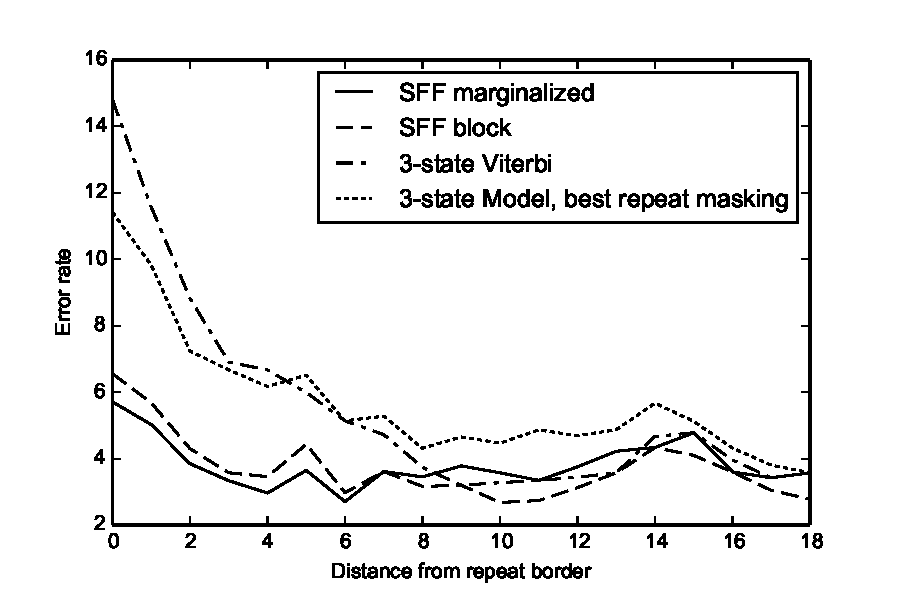
\includegraphics[width=\textwidth]{../figures/error_graph_overview.pdf}
\caption{Our methods and traditional methods}\label{FIGURE:SFFOVER}
\end{subfigure}%
\begin{subfigure}{0.5\textwidth}
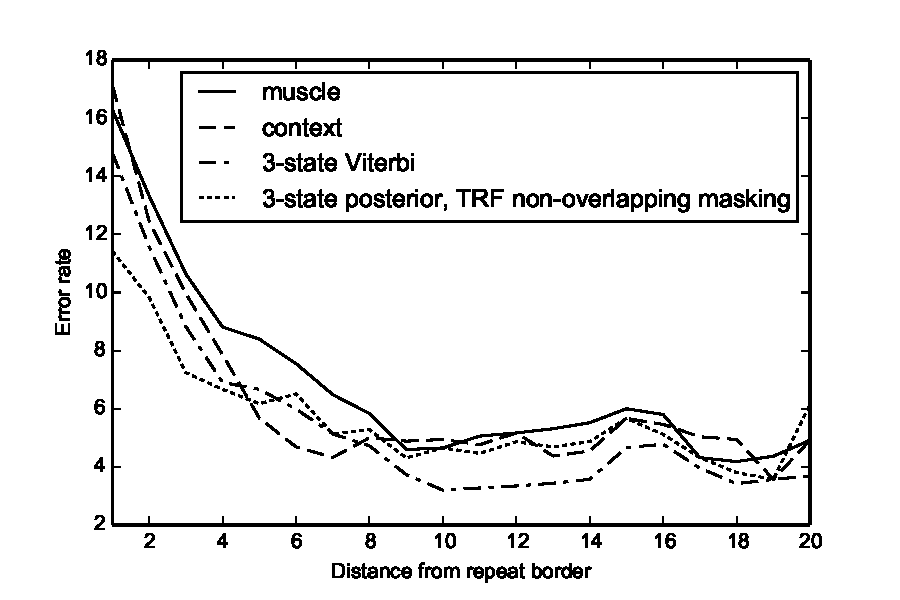
\includegraphics[width=\textwidth]{../figures/error_graph_other.pdf}
\caption{Other methods}\label{FIGURE:SFFOTHER}
\end{subfigure}%

\begin{subfigure}{0.5\textwidth}
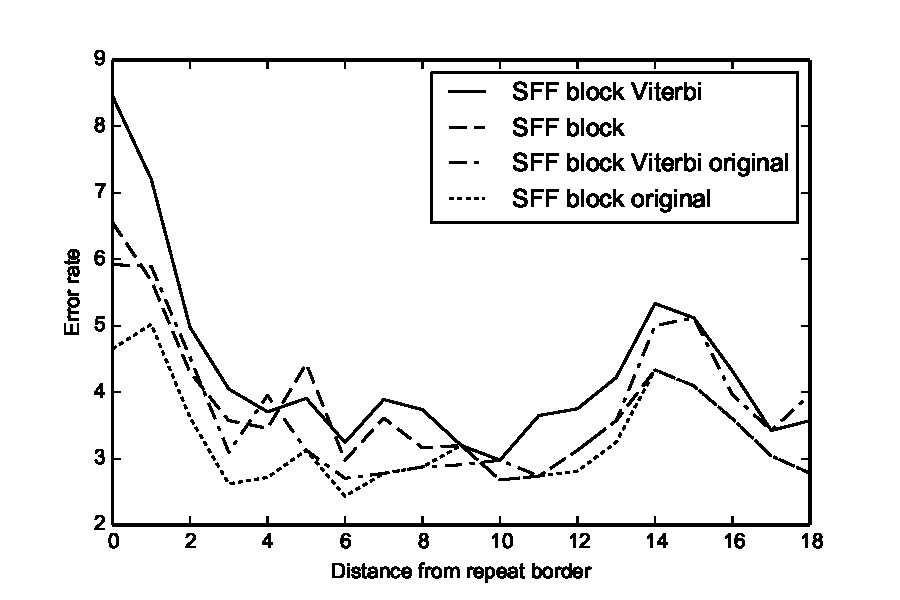
\includegraphics[width=\textwidth]{../figures/error_graph_sffblock.pdf}
\caption{Block decodings}\label{FIGURE:SFFBLOCKS}
\end{subfigure}%
\begin{subfigure}{0.5\textwidth}
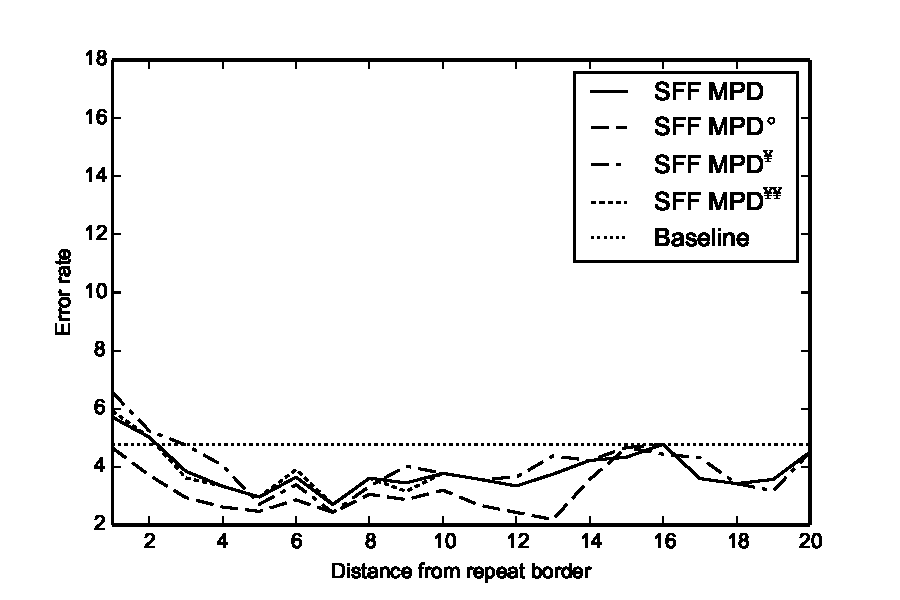
\includegraphics[width=\textwidth]{../figures/error_graph_marginalized.pdf}
\caption{Same method, different models}\label{FIGURE:SFFWEIRD}
\end{subfigure}%

\begin{subfigure}{0.5\textwidth}
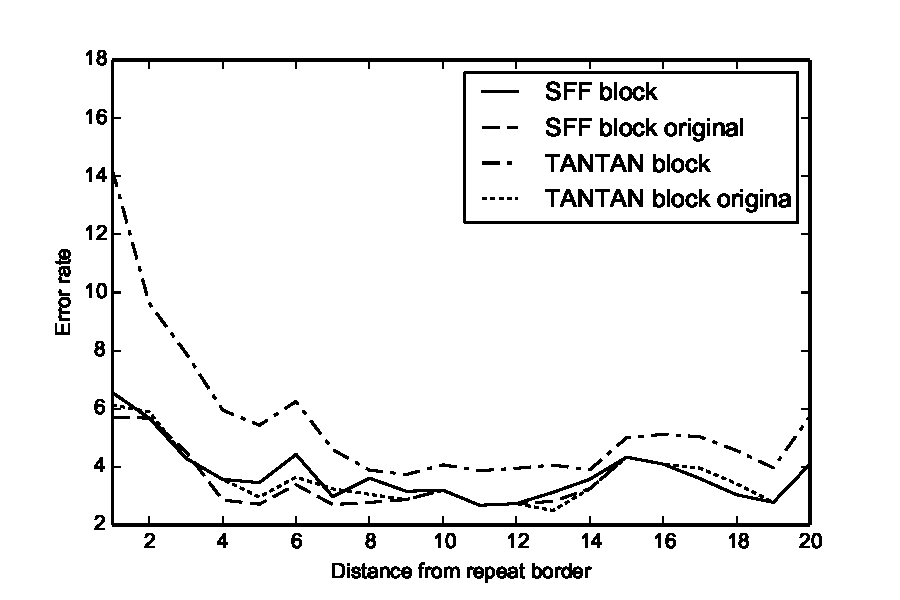
\includegraphics[width=\textwidth]{../figures/error_graph_sffvstantan.pdf}
\caption{Sunflower and TANTAN}\label{FIGURE:SFFTANTAN}
\end{subfigure}%
\begin{subfigure}{0.5\textwidth}
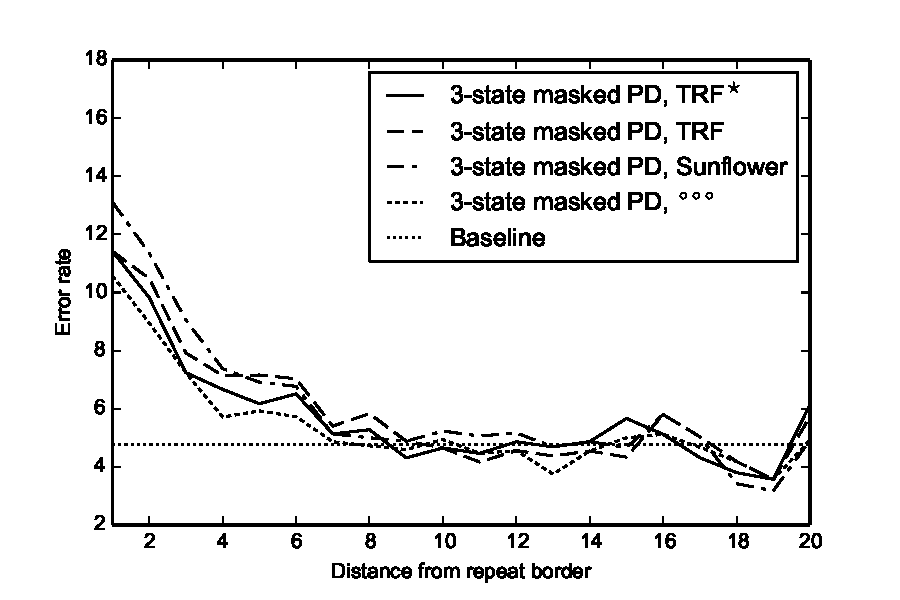
\includegraphics[width=\textwidth]{../figures/error_graph_3statemasking.pdf}
\caption{Different methods of masking}
\end{subfigure}%
\caption{
Relation between error rate and the distance from the nearest repeat. On the Y
axis is error rate of the algorithm; the number of incorrectly aligned columns.
On the X axis is the distance from the nearest repeat. Baseline is the overall
error rate, with no relation to the distance from the repeat border, for
3-state model with the Viterbi algorithm.
}\label{FIGURE:SFF_GRAPHS} 
\end{center}
\end{figure}

\section{Possible Improvements}

\begin{reformulate*}
Sem by som mohol napisat, ako by sa dal pouzit symetricky model s cyklom
stavov, alebo ako by sa dal ten cyklus stavov odstranit odstranenim jednej
hrany a pridanych n hran -- co je lepsie ako pridat n vrcholov.
\end{reformulate*}

\label{LastPage}
